\documentclass[letterpaper]{article}
\usepackage[utf8]{inputenc}
\usepackage[spanish]{babel}
\usepackage{amssymb, amsmath}
\usepackage{graphicx}
\usepackage{lipsum}
\usepackage{wasysym}
\usepackage{dsfont}
\usepackage[margin=1.5cm,
vmargin={2cm,1.3cm},
includefoot]{geometry}
\usepackage{setspace}
\usepackage{subcaption}
\usepackage{tocloft}
\usepackage{upgreek}
\usepackage{amsthm}
\usepackage{graphicx}
\usepackage{paralist}
\usepackage{fancyhdr}
\usepackage{lmodern}
\usepackage{tcolorbox}
\usepackage{color}
\usepackage{tikz}
\tcbuselibrary{skins,breakable}
\pagestyle{fancy}

\renewcommand{\headrulewidth}{0.4pt}
\renewcommand{\footrulewidth}{0.4pt}

\providecommand{\abs}[1]{\lvert#1\rvert}
\providecommand{\norm}[1]{\lVert#1\rVert}														  
\providecommand{\pint}[1]{<#1>}														  
\newcommand{\V}{\mathds{V}}

\newcommand{\W}{\mathds{W}}

\newcommand{\F}{\mathds{F}}

\newcommand{\tq}{ \quad \cdot  \backepsilon \cdot \quad }

\newcommand{\ld}{\lim\limits_{x \to 0^{+}}}

\newcommand{\li}{\lim\limits_{x \to 0^{-}}}

\newcommand{\la}{\lim\limits_{x \to a}}

\newcommand{\R}{\mathds{R}}

\renewcommand{\u}{\vec{u}}

\renewcommand{\v}{\vec{v}}

\newcommand{\Po}{\mathds{P}_2(\mathds{R})}

\renewcommand{\*}{\cdot}

\lhead{}

\chead{Matemáticas para las ciencas aplicadas II}
\rhead{ }

\newcommand{\Iden}{\begin{pmatrix}
		1 & 0 & 0\\
		0 & 1 & 0\\
		0 & 0 & 1 
\end{pmatrix}}
\newcommand{\T}{\begin{pmatrix}
		1 & 3 & 9 \\
		1 & 3 & 4 \\
		0 & 0 & 2 
\end{pmatrix} }

\makeatletter
\renewcommand*\env@matrix[1][*\c@MaxMatrixCols c]{%
	\hskip -\arraycolsep
	\let\@ifnextchar\new@ifnextchar
	\array{#1}}
\makeatother

\newtheorem{theorem}{Teorema}[section]
\newtheorem{corolario}[theorem]{Corolario}
\theoremstyle{definition}
\newtheorem{definition}{Definición}
\begin{document}
	
	\setlength{\unitlength}{1cm}
	\thispagestyle{empty}
	\begin{picture}(19,3)
	\put(-0.5,1.2){
\includegraphics[scale=.20]{unam1.png}}
	\put(16,1){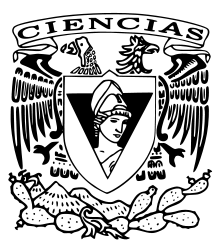
\includegraphics[scale=.29]{fciencias1.png}}
	\end{picture}
	
	\begin{center}
		\vspace{-114pt}
		\textbf{\large Matemáticas para las Ciencias II}\\
		\textbf{ Semestre 2020-2}\\
		Prof. Pedro Porras Flores\\
		Ayud. Irving Hernández Rosas \\
		\textbf{Tarea-examen I}\\[0.2cm]
		Kevin Ariel Merino Peña\footnote{317031326}\\ [0.2cm]
	\end{center}
	\vspace{-10pt}
	\rule{19cm}{0.3mm}
	
\section[Clase 23 de marzo]{Conjuntos abiertos}
\begin{theorem}
	Sean $ \vec{u} $ y $ \vec{v} $ dos vectores en $ \R^3 $ y sea $ \theta  \in \R$, donde $ 0 \leq \theta < \pi $ el ángulo entre ellos, entonces
	\[ <\vec{u}, \vec{v}> = \norm{\vec{u}}\norm{\vec{v}}\cos \theta \]
\end{theorem}
\begin{proof}
	Consideremos el triángulo formado por los vectores $ \vec{u}, \vec{v} $ y $ \vec{u} - \vec{v} $ de la ley de cosenos tenemos 
	\[ \norm{\vec{u}- \vec{v}}^2 = \norm{\vec{u}}^2 + \norm{\vec{v}}^2 - 2 \norm{\vec{u}}\norm{\vec{v}}\cos\theta \label{eq:norma} \tag{ \vernal } \]
	Por otro lado calculemos $ \norm{\vec{u} - \vec{v}}^2 $ esto es
	\begin{align*}
		\norm{\vec{u}- \vec{v}}^2 &= \pint{\u - \v, \u - \v} && \text{Por la definición de $ \norm{ x} $} \\
		\norm{\vec{u}- \vec{v}}^2 &= \pint{\u, \u - \v} + \pint{-\v, \u - \v} \\
		\norm{\vec{u}- \vec{v}}^2 &= \pint{\u, \u - \v} - \pint{-\v, \u - \v} \\
		\norm{\vec{u}- \vec{v}}^2 &= \pint{\u, \u } + \pint{\u, - \v} - \pint{\v, \u} -\pint{\v, \v} \\
		\norm{\vec{u}- \vec{v}}^2 &= \pint{\u, \u } + \pint{\u, - \v} - \pint{\u, \v} +\pint{\v, \v} \\
		\norm{\vec{u}- \vec{v}}^2 &= \norm{\u}^2 + \norm{\v}^2 - 2 \pint{\u, \v} \label{eq:otranorma} \tag{ \ascnode } \\
	\end{align*}
	Comparemos $ \ref{eq:norma} $ con $ \ref{eq:otranorma} $
	\[ -2\norm{\u}\norm{\v}\cos\theta = -2 \pint{\u, \v}  \implies \pint{\u, \v} = \norm{\u}\norm{\v}\cos\theta \quad \forall 0 \leq \theta < \pi \]
\end{proof}
\begin{corolario}[Desigualdad Cauchy-Schwarz]
	Para cualesquiera dos vectores $ \u  $ y $ \v $, se tiene que
	\[ \abs{\pint{\u, \v}} \leq \norm{\u}\norm{\v} \]
	La igualdad se da si y sólo si $ \u $ es múltiplo escalar de $ \v $ o uno de los vectores es 0
\end{corolario}
\begin{proof}
	Supongamos que $ \u $ no es múltiplo escalar  de $ \v $ y viceversa y que además ni $ \u $ ni $ \v $ son cero. Sabemos que\footnotetext[1]{Por nuestro curso de Matemáticas para las ciencias aplicadas I} \[ \abs{\cos} \leq 1 \quad \forall 0 \leq \theta \leq 2 \pi \label{eq:cosacotado} \tag{1} \]
	Por otro lado, sabemos que $ \pint{\u, \v} = \norm{\u}\norm{\v}\cos\theta $, tomando el valor absoluto, tenemos:
	\[ \abs{\pint{\u, \v}} = \norm{\u}\norm{\v}\abs{\cos \theta} \] si multiplicamos a $  (\ref{eq:cosacotado}) $ por $ \norm{\u}\norm{\v} $, entonces tenemos 
	\[ \abs{\pint{\u, \v}} = \norm{\u}\norm{\v}\abs{\cos \theta} \leq (1) \norm{\u}\norm{\v} = \norm{\u} \norm{\v} \]
	Por lo tanto $ \abs{\pint{\u,\v}} \leq \norm{\u}\norm{\v} $
\end{proof}
\newpage
\begin{theorem}[Desigualdad del triángulo]
	Sean $ \u, \v  \in \R^3$, entonces $ \norm{\u + \v} \leq \norm{\u} + \norm{\v} $
\end{theorem}
\begin{proof}
	De la desigualdad de \textit{ Cauchy-Schwarz} tenemos que, 
	\begin{align*}
		\abs{\u, \v} &\leq \norm{\u} \norm{\v} && \text{Por el corolario anterior}\\
		2\abs{\u, \v} &\leq 2\norm{\u} \norm{\v} && \text{como $ 2> 0 $}\\
		2\pint{\u, \v} &\leq 2 \abs{\pint{\u, \v}} && \text{Puesto que } \pint{\u, \v} \leq \abs{\pint{\u, \v}}\\
		2\pint{\u, \v} &\leq 2 \abs{\pint{\u, \v}} \leq  2\norm{\u}\norm{\v}  && \text{Por los dos últimos resltados}\\
		2\pint{\u, \v} &\leq  2\norm{\u}\norm{\v}  && \text{Por transitividad de la desigualdad }\\
		\norm{\u}^2 + \norm{\v}^2 + 2\pint{\u, \v} &\leq \norm{\u}^2 + \norm{\v}^2 + 2\norm{\u}\norm{\v}  && \text{Sumando en ambos lados } \norm{\u}^2 + \norm{\v}^2 \label{eq:desigualdad} \tag{2}\\
	\end{align*}
	Para concluir, observemos que $$ \norm{\u + \v} = \norm{\u}^2 + \norm{\v}^2 + 2 \pint{\u, \v} \label{eq:definicionInterno} \label{3} $$
	Luego, de $ (\ref{eq:desigualdad}), (\ref{eq:definicionInterno}) $ tenemos: 
	$ \norm{\u + \v} \leq \norm{\u}^2 + \norm{\v}^2 + 2 \norm{\u} \norm{\v} $, ahora tenemos 
	\begin{align*}
	\norm{\u+ \v}^2 & \leq (\norm{\u} + \norm{v})^2 && \text{factorizando el trinomio cuadrado pefecto}\\
	\norm{\u+ \v} & \leq \norm{\u} + \norm{v} && \text{Tomando la raíz cuadrada}
	\end{align*}
\end{proof}
\begin{corolario}
	Sean $ \u, \v \in \R^3 $, muestre que $ \norm{\u - \v} \geq \abs{\norm{\u} - \norm{\v}} $
\end{corolario}
\begin{definition}[Bola abierta]
	Sea $ \vec{x_0} $
\end{definition}
\end{document}